\documentclass{article}


\usepackage{arxiv}

\usepackage[utf8]{inputenc} % allow utf-8 input
\usepackage[T1]{fontenc}    % use 8-bit T1 fonts
\usepackage{hyperref}       % hyperlinks
\usepackage{url}            % simple URL typesetting
\usepackage{booktabs}       % professional-quality tables
\usepackage{amsfonts}       % blackboard math symbols
\usepackage{nicefrac}       % compact symbols for 1/2, etc.
\usepackage{microtype}      % microtypography
\usepackage{lipsum}
\usepackage{graphicx}
\usepackage[numbers]{natbib}

\usepackage{verbatim}
\usepackage{fancyvrb}
\usepackage{xcolor}
% see
% http://mirror.aut.ac.nz/CTAN/macros/latex/contrib/minted/minted.pdf
% on how to set the options during drafting and finalization:
\usepackage{minted} % needs `pdflatex -shell-escape blaom.tex`
% \usepackage[finalizecache=true]{minted} # once at end, needs same latex cmd
% \usepackage[frozencache=true]{minted}   # for submission with `pdflatex blaom.tex`
%\usepackage{authblk}
\usepackage{bm}
\usepackage{listings}

%To do:
%- [x] Formatting code in Julia style
%- [x] Fix the LinEtal2020 reference warning.
%- [x] Add tables to outputs of code samples
%- [x] Formatting authors and affiliations.
%- [ ] Fix z hat that is not visible in the paper

\title{MLJ: A Julia package for composable Machine Learning}

%\author[1,2,3]{Anthony D. Blaom}
%\author[3,4]{Franz Kiraly}
%\author[4]{Thibaut Lienart}
%\author[5]{Yiannis Simillides}
%\author[6]{Diego Arenas}
%\author[3,7]{Sebastian J. Vollmer}
%\affil[1]{University of Auckland}
%\affil[2]{New Zealand eScience Infrastructure}
%\affil[3]{Alan Turing Institute}
%\affil[4]{University College London}
%\affil[5]{Imperial College London}
%\affil[6]{University of St Andrews}
%\affil[7]{University of Warwick}

\author{
 Anthony D. Blaom \\
  %Department of Electrical Engineering\\
  University of Auckland, Alan Turing Institute, New Zealand eScience Infrastructure\\
  \texttt{anthony.blaom@gmail.com} \\
  \And
 Franz Kiraly \\
  %Department of Electrical Engineering\\
  University College London, Alan Turing Institute\\
  \texttt{fkiraly@turing.ac.uk} \\
  \And
 Thibaut Lienart \\
  %Department of Electrical Engineering\\
  Alan Turing Institute\\
  \texttt{tlienart@turing.ac.uk} \\
  \And
 Yiannis Simillides \\
  %Department of Electrical Engineering\\
  Imperial College London\\
  \texttt{ysimillides@imperial.ac.uk} \\
  \And
 Diego Arenas \\
  %School of Computer Science\\
  University of St Andrews\\
  \texttt{da60@st-andrews.ac.uk} \\
  \And
 Sebastian J. Vollmer \\
  %Department of Statistics\\
  Alan Turing Institute, University of Warwick\\
  \texttt{svollmer@turing.ac.uk} \\
}

\begin{document}
\maketitle

\begin{abstract}
MLJ (Machine Learing in Julia) is an open source software package
providing a common interface for interacting with machine learning
models written in Julia and other languages. It provides tools and
meta-algorithms for selecting, tuning, evaluating, composing and
comparing those models, with a focus on flexible model
composition. In this design overview we detail chief novelties of the
framework, together with the clear benefits of Julia over the dominant
multi-language alternatives.
 %\lipsum[1]
\end{abstract}

% keywords can be removed
\keywords{machine learning toolbox \and hyper-parameter optimization \and model composition \and Julia language \and pipelines}

\section{Introduction}

Statistical modelling, and the building of complex modelling pipelines, is a cornerstone of modern data science. Most experienced data scientists rely on high-level open source modelling toolboxes - such as sckit-learn \cite{Pedregosa2001}; \cite{Buitinck2013} (Python); Weka \cite{Holmes1994} (Java); mlr \cite{BischlEtal2016} and caret \cite{Kuhn2008} (R) - for quick blueprinting, testing, and creation of deployment-ready models. They do this by providing a common interface to atomic components, from an ever-growing model zoo, and by providing the means to incorporate these into complex work-flows. Practitioners are able to build increasingly sophisticated composite models, as exemplified in the strategies of top contestants in machine learning competitions such as Kaggle.

MLJ (Machine Learning in Julia) \cite{MLJ} is a toolbox written in Julia that provides a common interface and meta-algorithms for selecting, tuning, evaluating, composing and comparing machine model implementations written in Julia and other languages. More broadly, the MLJ project hopes to bring cohesion and focus to a number of emerging and existing, but previously disconnected, machine learning algorithms and tools of high quality, written in Julia. A welcome corollary of this activity will be increased cohesion and synergy within the talent-rich communities developing these tools.

In addition to other novelties outlined below, MLJ aims to provide first-in-class model composition capabilities. Guiding goals of the MLJ project have been usability, interoperability, extensibility, code transparency, and reproducibility.

\subsection{Why Julia?}

Nowadays, even technically competent users of scientific software will prototype solutions using a high-level language such as python, R, or MATLAB. However, to achieve satisfactory performance, such code typically wraps performance critical algorithms written in a second low-level language, such as C or FORTRAN. Through its use of an extensible, hierarchical system of abstract types, just-in-time compilation, and by replacing object-orientation with multiple dispatch, Julia solves the ubiquitous "two language problem" \cite{BezansonEtal2017}. With less technical programming knowledge, experts in a domain of application can get under the hood of machine learning software to broaden its applicability, and innovation can be accelerated through a dramatically reduced software development cycle.

As an example of the productivity boost provided by the single-language paradigm, we cite the DifferentialEquations.jl package \cite{RackauckasNie2017}, which, in a few short years of development by a small team of domain experts, became the best package in its class \cite{Rackauckas2017}.

Another major advantange of a single-language solution is the ability to automatically differentiate (AD) functions from their code representations. The Flux.jl package \cite{Innes2018}, for example, already makes use of AD to allow unparalleled flexibility in neural network design.

As a new language, Julia is high-performance computing-ready, and its superlative metaprogramming features allow developers to create domain-specific syntax for user interaction.

\subsection{Novelties}

In line with current trends in "auto-ML", MLJ's design is largely predicated on the importance of model composability. Composite models share all the behaviour of regular models, constructed using a new flexible "learning networks" syntax. Unlike the toolboxes cited above, MLJ's composition syntax is flexible enough to define stacked models, with out-of-sample predictions for the base learners, as well as more routine linear pipelines, which can include target transformations that are learned. As in mlr, hyper-parameter tuning is implemented as a model wrapper.

In MLJ, probabilistic prediction is treated as a first class feature, leveraging Julia's type sytem. In particular, unnecessary case-distinctions, and ambiguous conventions regarding the representation of probabilities, are avoided.

A user can connect models directly to tabular data in a manifold of in-memory and out-of-memory formats, and usability is enhanced through the introduction of "\textit{scientific types}" allowing the user to focus on the intended purpose of data ("continous", "ordered factor", etc) rather than particular machine type representations.

Finally, with the help of scientific types and the CategoricalArrays.jl package \cite{CategoricalArrays}, users are guided to create safe representations of categorical data, in which the complete pool of possible classes is embedded in the data representation, and classifiers preserve this information when making predictions!. This avoids a pain-point familiar in environments that simply recast categorical data using integers (e.g., scikit-learn): evaluating a classifier on the test target, only to find the test data includes classes not seen in the training data. Preservation of the original labels for these classes also facilitates exploratory data anaysis and interpretability.

\section{Scientific types}

To help users focus less on data representation (e.g., \texttt{Float32}, \texttt{CategoricalValue\{Char,UInt8\}} or \texttt{DataFrame}) and more on intended \textit{interpretation} (such as, "continuous", "ordered factor" and "table") MLJ articulates model data requirements, as well as data pre-processing tasks, using \textit{scientific types}. A scientific type is an ordinary Julia type (generally without instances) reserved for indicating how some data should be interpreted.

Some of these types (provided by an external package for re-use elsewhere) are shown in Figure \ref{fig:fig1}.

\begin{figure}
  \centering
  
\includegraphics[width=0.8\textwidth]{scitypesII}
  \caption{Part of the scientific type hierarchy.}
  \label{fig:fig1}
\end{figure}

To the scientific types, MLJ adds a specific \textit{convention} specifying a scientific type for every Julia object. The convention is expressed through a single method \texttt{scitype}. A \texttt{coerce} method to recasts machine types to have the desired scientific type (interpretation), and a \texttt{schema} method summarizes the machine and scientfic types of tabular data.

\begin{minted}[samepage]{julia}
    In[1]:  using MLJ, CategoricalArrays
            scitype(1.2)
    
    Out[1]: Continuous
    
    In[2]:  table = (age=[20, 13, 48], attempts=[10, 5, 6], query=["why", "what", "whom"])
            schema(table)
    
    Out[2]: -----------------------------------
            | _.names  | _.types | _.scitypes |
            -----------------------------------
            | age      | Int64   | Count      |
            | attempts | Int64   | Count      |
            | query    | String  | Textual    |
            -----------------------------------
    
            _.nrows = 3

    In[3]:  fixed_table = coerce(column_table, :age=>Continuous, :query=>Multiclass)
            schema(fixed_table)
    
    Out[3]: --------------------------------------------------------
            | _.names  | _.types                   | _.scitypes    |
            --------------------------------------------------------
            | age      | Float64                   | Continuous    |
            | attempts | Int64                     | Count         |
            | query    | CategoricalString{UInt32} | Multiclass{3} |
            --------------------------------------------------------
            
            _.nrows = 3
\end{minted}

%┌──────────┬─────────┬────────────┐
%│ _.names  │ _.types │ _.scitypes │
%├──────────┼─────────┼────────────┤
%│ age      │ Int64   │ Count      │
%│ attempts │ Int64   │ Count      │
%│ query    │ String  │ Textual    │
%└──────────┴─────────┴────────────┘

%┌──────────┬───────────────────────────┬───────────────┐
%│ _.names  │ _.types                   │ _.scitypes    │
%├──────────┼───────────────────────────┼───────────────┤
%│ age      │ Float64                   │ Continuous    │
%│ attempts │ Int64                     │ Count         │
%│ query    │ CategoricalString{UInt32} │ Multiclass{3} │
%└──────────┴───────────────────────────┴───────────────┘

Since scientific types are also Julia types, Julia's advanced type system means scientific types can be organized in a type hierarchy, and it is straightforward to check the compatibility of data with a model's scientific requirements and methods can be dispatched on scientific type just as they would on ordinary types.

\section{Connecting models directly to arbitrary data containers}

MLJ models generally expect features (and multivariate target data) to be tabular (rather than a raw matrix, for example). While there are many options for storing tabular data in Julia, both in memory or on disk, these can be accessed using a common interface provided by the Tables.jl package \cite{Quinn}. In MLJ, any Tables.jl-compatible table has scientific type \texttt{Table\{K\}}, where the type parameter \texttt{K} is the union of the column scientific types; most models allow scientific type for input features to be some subtype of \texttt{Table}.

While internally many models convert tabular data to matrices, a lightweight table wrapper for matrices provided by Tables.jl means that type coercion is skipped by the compiler in the case of matrix input (as readily verified using Julia's code inspection macro \texttt{@code\_llvm}).

\section{Finding the right model}

A model registry gives the user access to model metadata without the need to actually load code defining the model implementation. This metadata includes the model's data requirements (framed in terms of scientific types), the names and types of hyper-parameters, a brief document string, the url for the providing package, open source license and a load path to enable MLJ to locate the model interface code.

Such information allows users to match models to machine learning tasks, facilitating searches for an optimal model. For example, to find all supervised models making probabilistic predictions, compatible with input data \texttt{X} and target \texttt{y}, one defines a filter

\begin{minted}{julia}
    task(model) = matching(model, X, y) && model.prediction_type == 
    :probabilistic models(task)
\end{minted}

and lists the models with \texttt{models(task)}. 

\section{Flexible and compact work-flows for performance evaluation and tuning}

Evaluating the performance of some \texttt{model} object (specifying the hyper-parameters of some supervised learning algorithm) using some specified \texttt{resampling} strategy, and measured against some battery of performance \texttt{measures}, looks like this:

\begin{minted}{julia}
    evaluate(model, X, y, resampling=CV(nfolds=6), measures=[L2HingeLoss(), BrierScore()])
\end{minted}

%┌──────────────────────────────┬───────────────┬──────────────────────────────────%──────────────┐
%│ _.measure                    │ _.measurement │ _.per_fold                       %              │
%├──────────────────────────────┼───────────────┼──────────────────────────────────%──────────────┤
%│ L2HingeLoss                  │ 1.4           │ [0.485, 1.58, 2.06, 1.09, 2.18, %1.03]          │
%│ BrierScore{UnivariateFinite} │ -0.702        │ [-0.242, -0.788, -1.03, -0.545, %-1.09, -0.514] │
%└──────────────────────────────┴───────────────┴────────────────────────────────────────────────┘

As in mlr, hyper-parameter optimization is realized as a model wrapper, which transforms a base model into a "self-tuning" version of that model. That is, tuning is is abstractly specified before being executed. This allows tuning to be integrated into work-flows (learning networks) in multiple ways. A well-documented tuning interface \cite{MLJTuning} allows developers to easily extend available hyper-parameter tuning strategies.

We now give an example of syntax for wrapping a model called \texttt{forest\_model} in a random search tuning strategy, using cross-validation, and optimizing the mean square loss. The \texttt{model} in this case is a composite model with an ordinary hyper-parameter called \texttt{bagging\_fraction} and a nested hyper-parameter \texttt{atom.n\_subfeatures} (where \texttt{atom} is another model). The first two lines of code define ranges for these parameters.

\begin{minted}{julia}
    r1 = range(forest_model, :(atom.n_subfeatures), lower=1, upper=9)
    r2 = range(forest_model, :bagging_fraction, lower=0.4, upper=1.0)
    self_tuning_forest_model = TunedModel(model=forest_model,
                                          tuning=RandomSearch(),
                                          resampling=CV(nfolds=6),
                                          range=[r1, r2],
                                          measure=LPDistLoss(2),
                                          n=25)
\end{minted}

In this random search example default priors are assigned to each hyper-parameter but options exist to customize these. Both resampling and tuning have options for parallelization; Julia has first class support for both distributed and multi-threaded parallelism.

\section{A unified approach to probabilistic predictions and their evaluation}

MLJ puts probabilistic models and deterministic models on equal footing. Unlike most most frameworks, a supervised model is either \textit{probablistic} - meaning it's \texttt{predict} method returns a distribution object - \textit{or} it is \textit{deterministic} - meaning it returns objects of the same scientific type as the training observations. To use a probabilistic model to make deterministic predictions one can wrap the model in a pipeline with an appropriate post-processing function, or use additional \texttt{predict\_mean}, \texttt{predict\_median}, \texttt{predict\_mode} methods to deal with the common use-cases.

A "distribution" object returned by a probabilistic predictor is one that can be sampled (using Julia's \texttt{rand} method) and queried for properties. Where possible the object is in fact a \texttt{Distribution} object from the Distributions.jl package \cite{LinEtal2020}, for which an additional \texttt{pdf} method for evaluating the distribution's probability density or mass function will be implemented, and in addition to \texttt{mode}, \texttt{mean} and \texttt{median} methods (allowing MLJ's fallbacks for \texttt{predict\_mean}, etc, to work).

One important distribution \textit{not} provided by Distributions.jl is a distribution for finite labeled data (called \texttt{UnivariateFinite}) which additionally tracks all possible classes of the categorical variable it is modelling, and not just those observed in training data.

By predicting distributions, instead of raw probablities or parameters, MLJ avoids a common pain point, namely deciding and agreeing upon a convention about how these should be represented: Should a binary classifier predict one probability or two? Are we using the standard deviation or the variance here? What's the protocol for deciding the order of (unordered) classes? How should multi-target predictions be combined?, etc.

A case-in-point concerns performance measures (metrics) for probabilistic models, such as cross-entropy and Brier loss. All built-in probablisitic measures provided by MLJ are passed a distribution in their prediction slot.

For an overview on probabilistic supervised learning we refer to \cite{Gressmann2018}.

\section{Model interfaces}

MLJ provides a basic \texttt{fit/update/predict} interface to be implemented by new supervised models. For unsupervised models \texttt{predict} is replaced with \texttt{transform} and an optional \texttt{inverse\_transform} method. These methods operate on \textit{models} which are mutable structs storing hyper-parameters, and nothing else. This \textit{model interface} is purely functional for maximum flexibility. Presently the general MLJ user is encouraged to interact through a \textit{machine interface} sitting on top. See more on this below.

\subsection{The model interface}

In MLJ a \textit{model} is just a struct storing the hyper-parameters associated with some learning algorithm suggested by the struct name (e.g., \texttt{DecisionTreeClassifier}), and that is all. In the low-level, functional-style, model interface \textit{learned parameters} are not stored, only passed around. Learned parameters \textit{are} stored in machines (which additionally \textit{point} to the hyperparameters stored in a model); see below. The separation of hyper-parameters and learned parameters is essential to flexible model composition.

For supervised models the fit method has this signature:

\begin{minted}{julia}
    fit(model, verbosity, X, y)
\end{minted}

where \texttt{X} is training input and \texttt{y} the training target. The method outputs a triple, typically denoted \texttt{(fitresult, cache, report)}.

The \texttt{fitresult} stores the learned parameters, which must include everything needed by \texttt{predict} to make predictions, apart from \texttt{model} and new input data:

\begin{minted}{julia}
    predict(model, fitresult, X)
\end{minted}

The purpose of \texttt{cache} is to pass on "state" not included in the \texttt{fitresult} to an \texttt{update} method that the model implementer may optionally overload:

\begin{minted}{julia}
    update(model, verbosity, fitresult, cache, X, y)    
\end{minted}

This method is to be called instead of \texttt{fit} (and passed the \texttt{fitresult} and \texttt{cache} returned by the \texttt{fit} call) when retraining using identical data. (The data \texttt{X}, \texttt{y}, are included for implementer convenience.) It provides an opportunity for the model implementer to avoid unnecessary repetition of code execution. The three main use-cases are:

\begin{itemize}
    \item \textbf{Iterative models.} If the only change to a random forest model is an increase in the number of trees by ten, for example, then not all trees need to be retrained; only ten new trees need to be trained. If a "self-tuning" model has been fit (i.e., tuned) using 70 iterations of Tree Parzen optimization, then adding 20 more iterations should build on the existing surrogate objective function, not ignore the existing tuning history.
    \item \textbf{Data preprocessing.} Avoid overheads associated with data preprocessing, such as coercion of data into an algorithm-specific type.
    \item \textbf{Smart training of composite models.} When tuning a simple transformer-predictor pipeline model using a holdout set, for example, it is unecessary to retrain the transformer if only the predictor hyper-parameters change. MLJ implements "smart" retraining of composite models like this by defining appropriate \texttt{update} methods.
\end{itemize}

In the future MLJ will add an \texttt{update\_data} method to support models that can cary out on-line learning.

\subsection{The machine interface}

The general MLJ user trains models through its machine interface. This makes some work-flows more convenient, but more significantly, introduces a syntax closely aligned with that for model composition (see below).

A \textit{machine} is a mutable struct that binds a model to data at construction

\begin{minted}{julia}
    mach = machine(model, X, y)    
\end{minted}

When the user calls \texttt{fit!(mach, rows=...)} the \texttt{fitresult}, \texttt{cache} and \texttt{report} variables generated by lower-level calls to \texttt{fit} or \texttt{update}, are stored or updated in the machine struct, \texttt{mach}, with the training being optionally restricted to the specified rows of data. To retrain with new hyper-parameters, the user simply mutates
\texttt{model} and repeats the \texttt{fit!} call.

Syntax for predicting using a machine is \texttt{predict(mach, Xnew)}.

\section{Flexible model composition}

Several limitations surrounding model composition are increasingly evident to users of the dominant machine learning software platforms. The basic model composition interfaces provided by the toolboxes mentioned in the Introduction all share one or more of the following shortcomings, which do not exist in MLJ:

\begin{itemize}
    \item Composite models do not inherit all the behavior of ordinary models.
  \item Composition is limited to linear (non-branching) pipelines.
  \item Supervised components in a linear pipeline can only occur at the end of the pipeline.
  \item Only static (unlearned) target transformations/inverse transformations are supported.
  \item Hyper-parameters in homogeneous model ensembles cannot be coupled.
  \item Model stacking, with out-of-sample predictions for base learners, cannot be implemented.
  \item Hyper-parameters and/or learned parameters of component models are not easily inspected or manipulated (in tuning algorithms, for example).
\end{itemize}

We now sketch MLJ's composition API, referring the reader to \cite{Blaom_I} for technical details, and to the MLJ documentation \cite{MLJdocs}; \cite{MLJtutorials} for examples that will clarify how the composition syntax works in practice.

Note that MLJ also provides "canned" model composition for common use cases, such as non-branching pipelines and homogeneous ensembles, which are not discussed further here.

Specifying a new composite model type is in two steps, \textit{prototyping} and \textit{export}.

\subsection{Prototyping}

In prototyping the user defines a so-called \textit{learning network}, by effectively writing down the same code she would use if composing the models "by hand". She does this using the machine syntax, with which she will already be familiar, from the basic \texttt{fit!}/\texttt{predict} work-flow for single models. There is no need for the user to provide production training data in this process. A dummy data set suffices, for the purposes of testing the learning network as it is built.

\begin{figure}
  \centering
  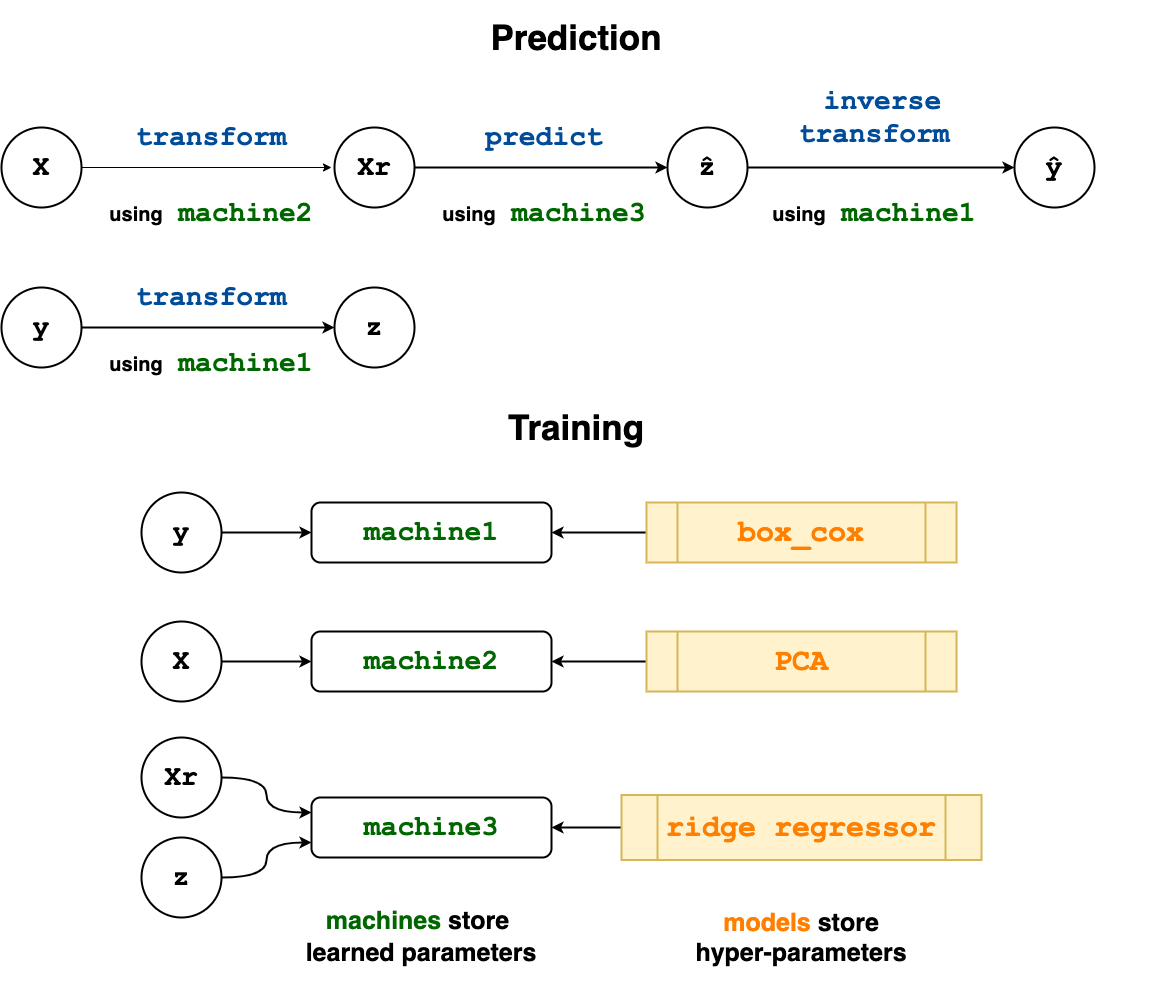
\includegraphics[width=0.8\textwidth]{target_transformerVERTICAL}
  \caption{Specifying prediction and training flows in a simple learning network. The network shown combines a ridge regressor with a learned target transformation (Box Cox).}
  \label{fig:fig2}
\end{figure}

The upper panel side of Figure \ref{fig:fig2} illustrates a simple learning network in which a continuous target \texttt{y} is "normalized" using a learned Box Cox transformation, producing \texttt{z}, while PCA dimension reduction is applied to some features \texttt{X}, to obtain \texttt{Xr}. A Ridge regressor, trained using data from \texttt{Xr} and \texttt{z}, is then applied to \texttt{Xr} to make a target prediction \texttt{\^{z}}. To obtain a final prediction \texttt{\^{y}}, we apply the \textit{inverse} of the Box Cox transform, learned previously, to \texttt{\^{z}}. 

The lower "training" panel of the figure shows the three machines which will store the parameters learned in training - the Box Cox exponent and shift (\texttt{machine1}), the PCA projection (\texttt{machine2}) and the ridge model coefficients and intercept (\texttt{machine3}). The diagram additionally indicates where machines should look for training data, and where to accesses model hyper-parameters (stored in \texttt{box\_cox}, \texttt{PCA} and \texttt{ridge\_regressor}).

The only syntactic difference between composing "by hand" and building a learning network is that the training data must be wrapped in "source nodes" (which can be empty if testing is not required). Each data "variable" in the manual workflow becomes instead a node of a directed acyclic graph encoding the composite model architecture. Nodes are callable, with a node call triggering lazy evaluation of the \texttt{predict}, \texttt{transform} and other operations in the network. Instead of calling \texttt{fit!} on every machine, a single call to \texttt{fit!} on a \textit{node} triggers training of all machines needed to call that node, in appropriate order. As mentioned earlier, training such a node is "smart" in the sense that hyper-parameter changes to a model only trigger retraining of necessary machines. So, for example, there is no need to retrain the Box Cox transformer in the preceding example if only the ridge regressor hyper-parameters have changed.

The syntax, then, for specifying the learning network shown in Figure \ref{fig:fig2} looks like this:

\begin{minted}[escapeinside=||,mathescape=true, samepage]{julia}
    X = source(X_dummy)        # or just source()
    y = source(y_dummy)        # or just source()
    
    machine1 = machine(box_cox, y)
    z = transform(machine1, y)
    
    machine2 = machine(PCA, X)
    Xr = transform(machine2, X)
    
    machine3 = machine(ridge_regressor, Xr, z)
    |$\hat{\texttt{z}}$| = predict(machine3, Xr)
    
    ŷ = inverse_transform(machine1, |$\hat \texttt{z}$|)
    
    fit!(ŷ)  # to test training on the dummy data
    ŷ()      # to test prediction on the dummy data
\end{minted}
%\^{z}
%$\hat{z}$
%ẑ = predict(machine2, X)
%ŷ = inverse_transform(machine1, ẑ)

Note that the machine syntax is a mechanism allowing for multiple nodes to point to the same learned parameters of a model, as in the learned target transformation/inverse transformation above. They also allow multiple nodes to share the same model (hyper-parameters) as in homogeneous ensembles. And different nodes can be accessed during training and "prediction" modes of operation, as in stacking.

\subsection{Export}

In the second step of model composition, the learning network is "exported" as a new stand-alone composite model type, with the component models appearing in the learning network becoming default values for corresponding hyper-parameters (whose values are themselves models). This new type (which is unattached to any particular data) can be instantiated and used just like any other MLJ model (tuned, evaluated, etc). Under the hood, training such a model builds a learning network, so that training is "smart". Defining a new composite model type requires generating and evaluating code, but this is readily implemented using Julia's meta-programming tools, i.e., executed by the user with a simple macro call.

\section{Future directions}

Here is a selection of future work planned or in progress:

\begin{itemize}
    \item \textbf{Supporting more models}. Proofs of concept already exist for interfacing pure-Julia deep learning and probabilistic programming models.
    \item \textbf{Enhancing core functionality}. Add more tuning strategies, in particular, Bayesian methods and AD-powered gradient descent.
   \item \textbf{Broadening Scope}. Adding resampling strategies and tools for dealing with time series data, and for dealing with sparse data relevant in natural language processing.
   \item \textbf{Scalability}. Add DAG scheduling for learning network training
\end{itemize}

A more comprehensive road map is linked from the MLJ repository \cite{MLJ}.

\section*{Acknowledgements}

We acknowledge valuable conversations with Avik Sengupta, Mike Innes, mlr author Bernd Bischl, and IQVIA's Yaqub Alwan and Gwyn Jones. Seed funding for the MLJ project has been provided by the Alan Turing Institute's Tools, Practicies Systems programme, with special thanks to Dr James Hethering, its former Programme Director, and Katrina Payne. Mathematics for Real-World Systems Centre for Doctoral Training at the University of Warwick provided funding for students exploring the Julia ML ecosystem, who created an intial proof-of-concept.

\textbf{Code contributors}. D. Aluthge, D. Arenas, E. Barp, C. Bieganek, A. Blaom, G. Bohner, M. K. Borregaard, D. Buchaca, V. Churavy, H. Devereux, M. Giordano, J. Hoffimann, T. Lienart, M. Nook, Z. Nugent, S. Okon, P. Oleśkiewicz, J. Samaroo, A. Shridar, Y. Simillides, A. Stechemesser, S. Vollmer.

\bibliographystyle{unsrtnat}
\bibliography{references}  %%% Remove comment to use the external .bib file (using bibtex).
%%% and comment out the ``thebibliography'' section.


\end{document}
